\section{Evaluations}
\label{sec:eval}

We conducted three evaluations to show the effectiveness of our approach in
generating regression tests that achieve a high coverage of the code under test. 
Our empirical results show that our approach is scalable and can automatically generate
tests for large real-word applications without any manual efforts. In our evaluations, 
we use ten .NET 2.0 framework base class libraries as subject applications. We next describe
the research questions addressed in our evaluation and present our evaluation results.

\begin{figure*}[t]
\centering
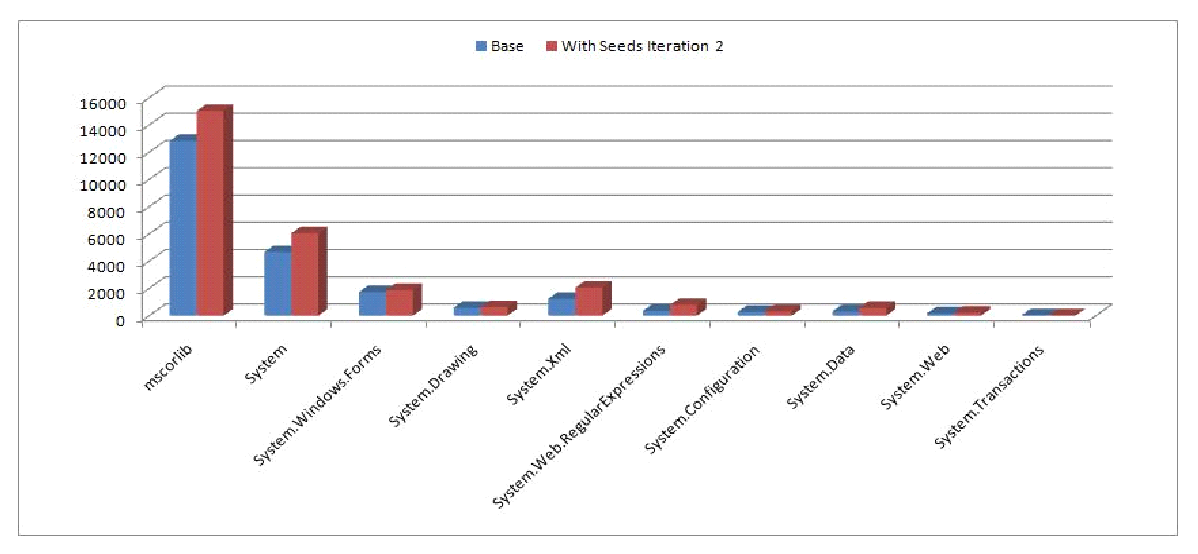
\includegraphics[scale=0.70,clip]{figs/RQ2_1.eps}\vspace*{-1ex}
\caption{Comparison of base coverage and coverage achieved by regression tests of Mode 4 (WithSeeds Iteration 2).} \label{fig:rq2}
\end{figure*}

%---------------------------------------------------------------------------------------
\subsection{Research Questions}
\label{sec:research}

We address the following three research questions in our evaluations.

\begin{itemize}
\item RQ1: Can our approach handle large real-world applications in automatically generating
regression tests that achieve a high coverage of the code under test? 
\item RQ2: Do seed tests help achieve higher coverage of the code under test than without using seed tests?
\item RQ3: Can more machine power help generate new regression tests that can achieve
more coverage of the code under test?
\end{itemize}

%---------------------------------------------------------------------------------------
\subsection{Subject Applications}

We used ten .NET 2.0 framework base class 
libraries\footnote{\url{http://msdn.microsoft.com/en-us/library/ms229335.aspx}} as subject applications in our
evaluations. We selected these libraries for two main reasons. First, these libraries
are the core libraries of .NET framework and are used by thousands
of developers and millions of end users. Therefore, these libraries can
represent real-world applications. Second, these libraries are extensively
tested over several years and are suitable for generating regression tests. 
Table~\ref{tab:subjects} shows the ten libraries used in our 
evaluations and their characteristics such as the number of classes and 
methods. The table shows that these libraries include $0$ LOC with
$0$ classes and $0$ methods.

\setlength{\tabcolsep}{1pt}
\begin{table}[t]
\begin{SmallOut}
\begin{CodeOut}
\begin{center}
\begin {tabular} {|l|c|c|c|}
\hline
\textbf{.NET libraries} & \textbf{LOC} & \textbf{\# public} & \textbf{\# public}\\ 
 & & \textbf{classes} & \textbf{methods}\\ 
\hline
\hline  mscorlib & 185K & 1440 & 17800 \\
\hline  System &  & & \\
\hline  System.Windows.Forms & & & \\
\hline  System.Drawing & & & \\
\hline  System.Xml & 150K & 686 & 9920 \\
\hline  System.Web.RegularExpressions & & & \\
\hline  System.Configuration & & & \\
\hline  System.Data & 196K & 648 & 11550 \\
\hline  System.Web &  & & \\
\hline  System.Transactions & & & \\
\hline \textbf{TOTAL} &  &  &   \\
\hline
\end{tabular}
\end{center}
\end{CodeOut}
\end{SmallOut}\vspace*{-4ex}
\centering \caption {\label{tab:subjects}Ten .NET framework base class libraries used in our evaluations}
\end{table}

%---------------------------------------------------------------------------------------
\subsection{Evaluation Setup}

In our approach, we used nine machines that can be classified into three 
configuration categories. On each machine, we launched multiple Pex
processes. The number of processes launched on a machine is
based on the configuration of the machine. For example, on an
eight core machine, we launched seven Pex processes. Each Pex process
was exploring one class (including multiple PUTs) at a time.
Table~\ref{tab:mconfig} shows all three configuration
categories. The table also shows the number of machines
of each configuration and the number of Pex processes launched on each machine.

\setlength{\tabcolsep}{1pt}
\begin{table}[t]
\begin{SmallOut}
\begin{CodeOut}
\begin{center}
\begin {tabular} {|l|c|c|}
\hline
\textbf{Machine Configuration} & \textbf{\# of} & \textbf{\# of} \\  
 & \textbf{machines} & \textbf{processes}\\  
\hline
\hline  Xeon 2 CPU @ 2.50 GHz, 8 cores & 1 & 7\\
				16 GB RAM & & \\
\hline  Quad core 2 CPU @ 1.90 GHz, 8 cores& 2 & 7\\
				8 GB RAM & & \\
\hline  Intel Xeon CPU @2.40 GHz, 2 cores& 6 & 1\\
				1 GB RAM & & \\
\hline
\end{tabular}
\end{center}
\end{CodeOut}
\end{SmallOut}\vspace*{-4ex}
\centering \caption {\label{tab:mconfig}Three categories of machine configurations used in our evaluations.}
\end{table}

As we used .NET framework base class libraries in our evaluations, the generated tests
may invoke method calls that can result in the corruption of the machine. Therefore,
while executing the code during exploration of PUTs or while running generated tests,
we created a sand-box with the ``Internet'' security permission. This permission
represents the default policy permission set for the content from an unknown origin.
This permission blocks all operations that involve environment interactions such
as file creations or registry accesses by throwing \CodeIn{SecurityException}.
Since we use sand-box in our evaluations, the reported coverage
is lower than the actual coverage that can be achieved by our generated regression
tests.

To address our research questions, we first created a base line in terms
of the code coverage achieved by the seed tests, referred to as \emph{base coverage}. 
In our evaluations, we use block coverage~\cite{} as a coverage 
criteria. We report our coverage in terms of the number of blocks covered in the code under test. The reason
for not able to present the coverage as a percentage
of the number of blocks to the total number of blocks is 
that we do not know how many blocks in the code under test are actually reachable.

We next generated regression tests in four different modes.
In Mode 1 (referred to as \emph{WithoutSeeds Iteration 1}), we generated
regression tests without using seed tests for one iteration. In Mode 2
(referred to as \emph{WithoutSeeds Iteration 2}), we generated regression 
tests without using seed tests for two iterations. The regression tests 
generated in Mode 2 are a super set of the regression tests generated
in Mode 1. In Mode 3 (referred to as \emph{WithSeeds Iteration 1}), 
we generated regression tests with using seed tests for one iteration. Finally, in 
Mode 4 (referred to as \emph{WithSeeds Iteration 2}), we generated
regression tests with using seed tests for two iterations. Modes 1
and 3 took one and half day for generating tests, whereas Modes 2
and 4 took three days since these modes correspond to Iteration 2.

%---------------------------------------------------------------------------------------
\subsection{RQ1: Generated Regression Tests}

We next address the first research question of whether our approach can 
handle large real-world applications in automatically generating regression
tests. This research question helps to show that our approach can be used 
in practice and can address scalability issues in generating regression tests for large applications.
We first present the statistics after each phase in our approach
and next present the number of regression tests generated in each mode.

In the capture phase, our approach recorded $\approx$1.50 GB C\# source
code (including 433,809 traces) of dynamic traces for the ten libraries.
The average trace length includes $21$ method calls and 
the maximum trace length includes $52$ method calls. As our capture phase transforms 
each dynamic trace into a PUT and a seed test, the capture phase resulted in 433,809
PUTs and 433,809 seed tests. 

In the minimize phase, our approach uses static analysis to filter out 
duplicate PUTs. Our static analysis took 45 minutes and resulted in 68,575 unique PUTs. 
Our approach uses dynamic analysis to filter our duplicate seed tests.
Our dynamic analysis took 5 hours and resulted in 128,185 unique seed tests.
These results show that there are a large number of duplicate PUTs
and seed tests, and show the significance of our minimize phase. 
We next measured the block coverage achieved by these 128,185 unique seed tests
in the code under test and used this coverage as \emph{base coverage}.
These tests covered 22,111 blocks in the code under test.

Table~\ref{tab:gentests} shows the number of regression tests generated in each mode
along with the number of covered blocks. The table also shows the percentage of increase
in the number of blocks compared to the base coverage. As shown in results,
in Mode 4 (WithSeeds Iteration 2), our approach achieved 24.3\% higher
coverage than the base coverage. Figure~\ref{fig:rq2} shows detailed
comparison of coverages between base coverage and Mode 4 for each library.
In the figure, x-axis represent the library and y-axis represent the number
of covered blocks. As we use seed tests during our exploration, the 
coverage achieved is either the same or higher than the base coverage.
However, our approach has achieved significant higher coverages than
base coverage for libraries mscorlib and System. The primary reason is that most of the classes in these
libraries are stateless and do not require environment interactions.
The results show that our approach can handle large real-world applications 
and can generate large number of regression tests that achieve a high coverage of the code under test.

\setlength{\tabcolsep}{1pt}
\begin{table}[t]
\begin{SmallOut}
\begin{CodeOut}
\begin{center}
\begin {tabular} {|l|c|c|c|}
\hline
\textbf{Mode} & \textbf{\# of} & \textbf{\# of covered} & \textbf{\% of increase}\\  
 & \textbf{Tests} & \textbf{blocks} & \textbf{from base}\\  
\hline
\hline  WithoutSeeds Iteration 1 & 248,306 & 21,920 & 0\%\\
\hline  WithoutSeeds Iteration 2 & 412,928 & 23,176 & 4.8\%\\
\hline  WithSeeds Iteration 1 & 376,367 & 26,939 & 21.8\%\\
\hline  WithSeeds Iteration 2 & 501,799 & 27,485 & 24.3\%\\
\hline
\end{tabular}
\end{center}
\end{CodeOut}
\end{SmallOut}\vspace*{-4ex}
\centering \caption {\label{tab:gentests}Generated regression tests.}
\end{table}

%---------------------------------------------------------------------------------------
\subsection{RQ2: Using Seed Tests}

We next address the second research question of whether seed tests help achieve 
higher code coverage compared to without using seed tests. To address this question,
we compare the coverages achieved by generated tests in Modes 2 (WithoutSeeds Iteration 2) and 4 (WithSeeds
Iteration 2) along with the base coverage. Figure~\ref{fig:rq3} shows the 
comparison results for each library. As shown in the figure, Mode 4 has
always achieved higher coverage than Mode 2. On average, Mode 4 achieved 
18.6\% higher coverage than Mode 2. These results show that seed tests are 
helpful in achieving higher code coverages.

\begin{figure*}[t]
\centering
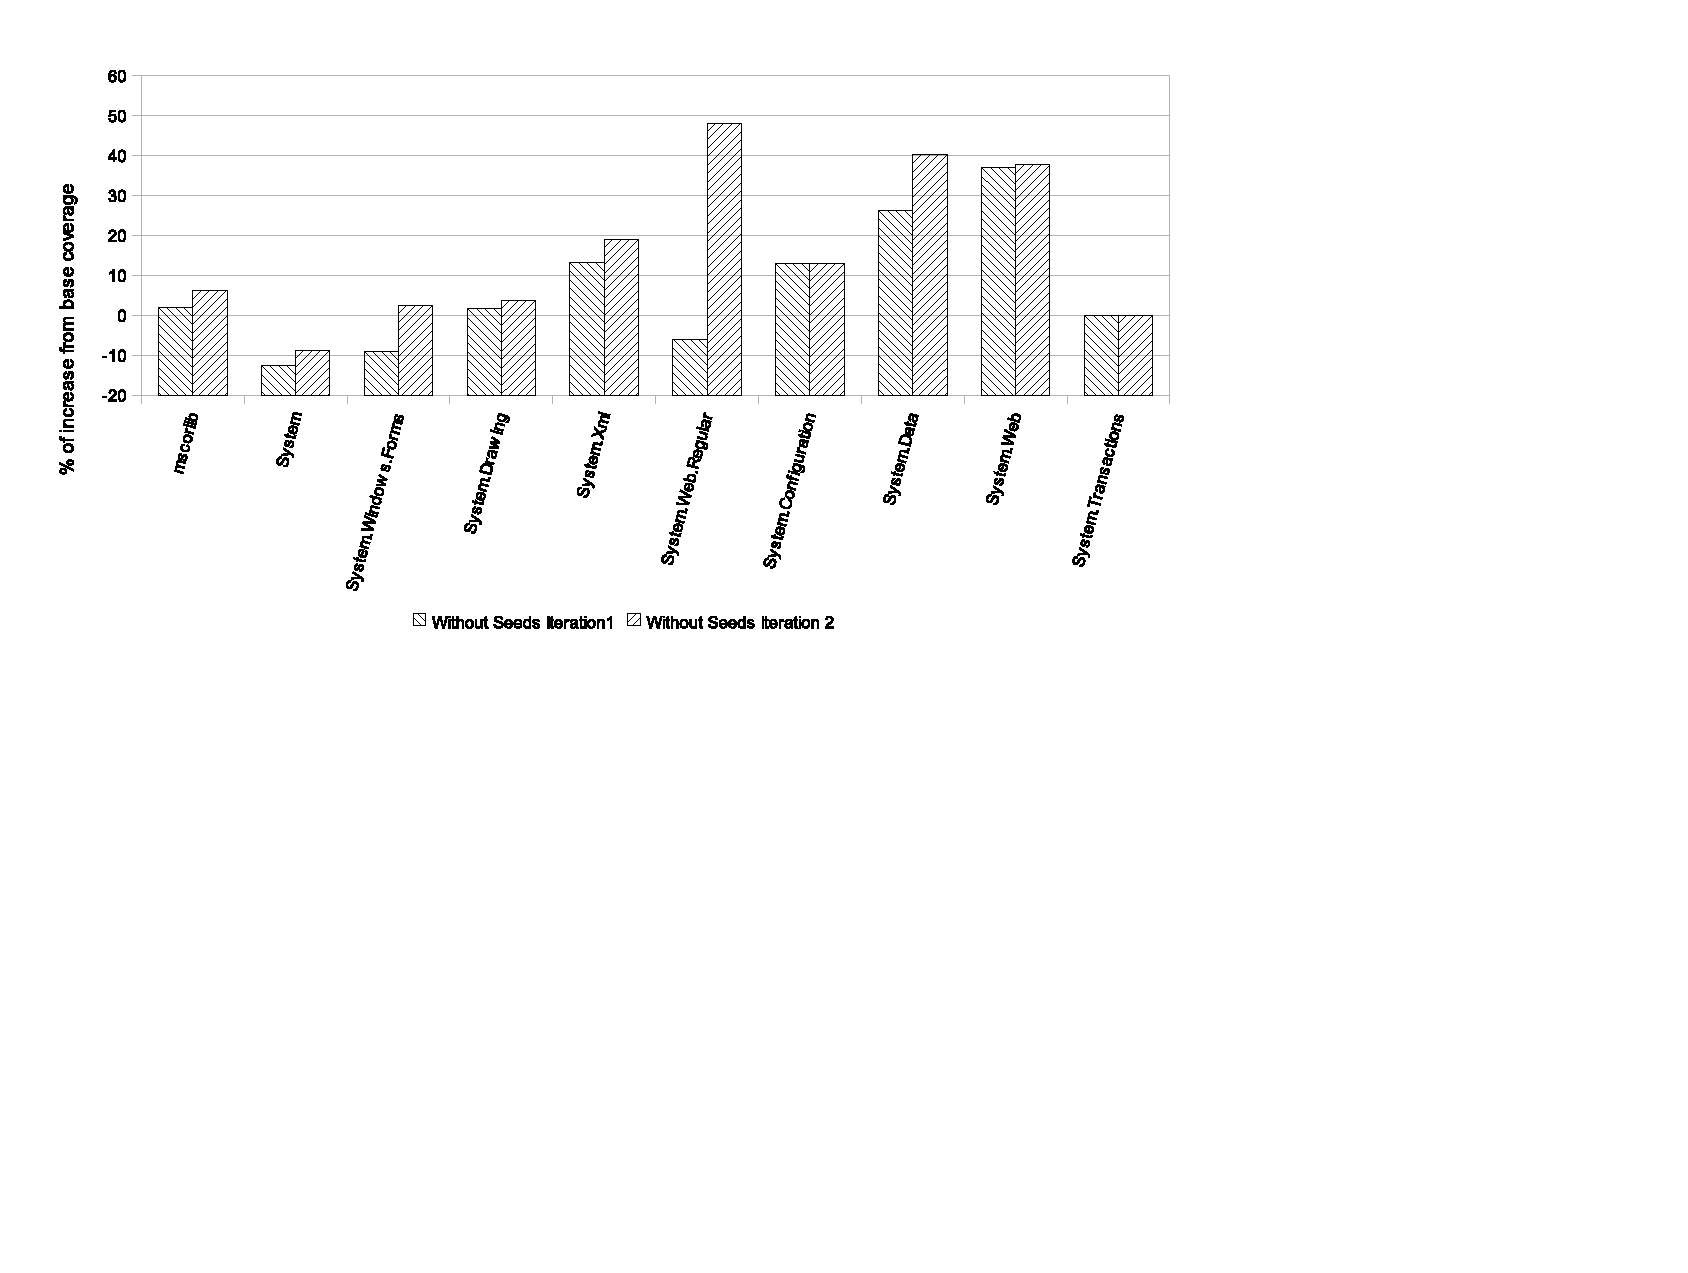
\includegraphics[scale=0.70,clip]{figs/RQ3_1.eps}\vspace*{-1ex}
\caption{Comparison of code coverages achieved by base, Modes 2 (WithoutSeeds Iteration 2) and 4 (Withseeds Iteration 2).} \label{fig:rq3}
\end{figure*}

%---------------------------------------------------------------------------------------
\subsection{RQ3: Using More Machine Power}

We next address the third research question of whether more machine power helps to
achieve more coverage. This research question helps to show that additional
coverage can be achieved in further iterations of our approach.
To address this question, we compare coverages achieved in Mode 1 (WithoutSeeds Iteration 1) with
Mode 2 (WithoutSeeds Iteration 2), and Mode 3 (WithSeeds Iteration 2) with
Mode 4 (WithSeeds Iteration 2). 

Figure~\ref{fig:rq41} shows the comparison results of Mode 1 with Mode 2 for all libraries. 
On average, Mode 2 achieved 5.73\% higher coverage than Mode 1. This result show
that our approach can achieve additional coverage in further iterations. However,
the coverage from Mode 1 to Mode 2 is not doubled. 
The primary reason is that it gets harder to cover new blocks in further iterations.

Figure~\ref{fig:rq42} shows the comparison results of Mode 3 with Mode 4. On average, 
Mode 4 achieved 2.0\% higher coverage than Mode 3. As shown, the increase in
coverage from Mode 3 to Mode 4 is less than the increase in the coverage from Mode 1
to Mode 2. This difference is due to seed tests that help achieve higher coverage
during Mode 3, leaving more harder blocks to be covered in Mode 4. In summary,
the results show that further iterations can help generate new regression
tests that can achieve more coverage.

\begin{figure*}[t]
\centering
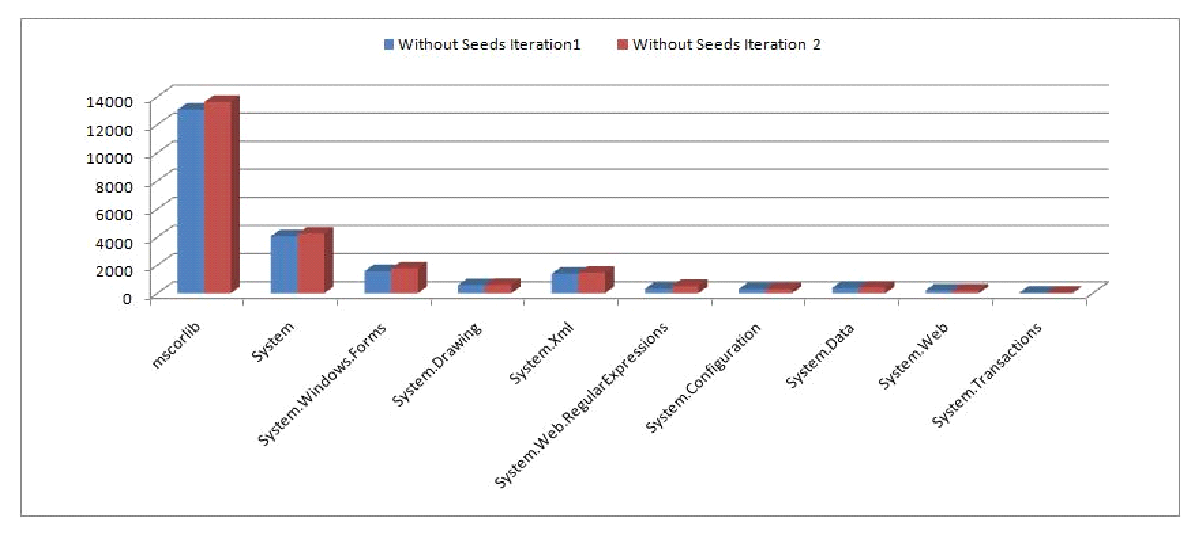
\includegraphics[scale=0.70,clip]{figs/RQ4_1_1.eps}\vspace*{-1ex}
\caption{\label{fig:rq41}Comparison of code coverages achieved by Modes 1 (WithoutSeeds Iteration 1) and 2 (WithoutSeeds Iteration 2).} 
\end{figure*}


\begin{figure*}[t]
\centering
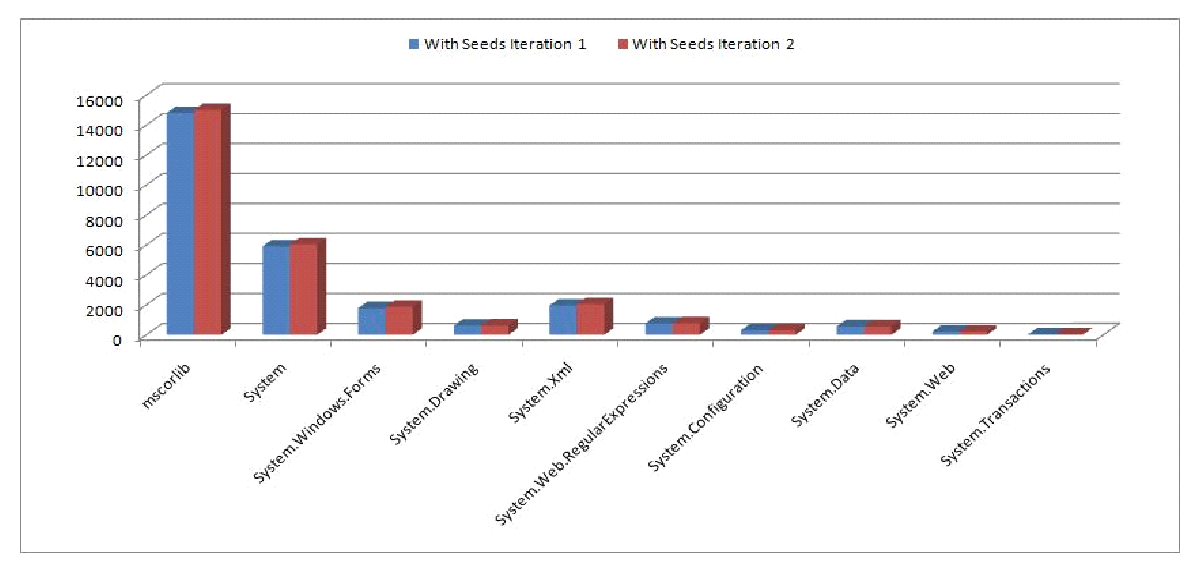
\includegraphics[scale=0.70,clip]{figs/RQ4_2_1.eps}\vspace*{-1ex}
\caption{\label{fig:rq42}Comparison of code coverages achieved by Modes 3 (WithSeeds Iteration 1) and 4 (Withseeds Iteration 2).}
\end{figure*}

%---------------------------------------------------------------------------------------
\subsection{Real Defects}

%Our approach automatically generates test scenarios from dynamic traces. We use these test scenarios
%in generating PUTs and then generating regression tests on a stable versions. These regression tests
%can be used on future versions to detect regression faults. In our approach, we cannot detect
%defects in the version on which regression tests generated because of lack of test oracles. However,
%we identify that many exceptions are observed while generating regression tests on the version.
%We next describe the raised exceptions and describe more about the defects detected.